\documentclass[a4paper,12pt]{article}
\usepackage[french]{babel} 
\usepackage[T1]{fontenc}
%\usepackage[ansinew]{inputenc}
\usepackage[utf8]{inputenc}
\usepackage[top=3cm, bottom=3cm, left=2.3cm,right=2cm]{geometry}
\usepackage{graphicx}
\usepackage{color}
\usepackage{listings}
%\usepackage{marvosym}
%\usepackage{yfonts}
\usepackage[normalem]{ulem}
\usepackage{verbatim}
\usepackage{listings}
\usepackage{float}
%\renewcommand{\thesection}{\arabic{section}}
\usepackage{array} % pour les tableaux
\usepackage{amsmath} % pour les équations
\usepackage{float}
\usepackage{hyperref}	% crée des liens dans le pdf
\hypersetup{					% colorise les liens du pdf
  colorlinks=true,
  urlcolor=black
	citecolor=black,
  linkcolor=black,
  urlcolor=blue
}
\usepackage{url}			% change la police des url (utilisation : \url{http://asdf.ch})
\definecolor{dkgreen}{rgb}{0,0.6,0}
\definecolor{gray}{rgb}{0.5,0.5,0.5}
\definecolor{mauve}{rgb}{0.58,0.01,0.82}
%[babel=true]
\usepackage{csquotes}
\lstset{ %
  language=C,                % the language of the code
  basicstyle=\footnotesize,           % the size of the fonts that are used for the code
  numbers=left,                   % where to put the line-numbers
  numberstyle=\tiny\color{gray},  % the style that is used for the line-numbers
  stepnumber=1,                   % the step between two line-numbers. If it's 1, each line 
                                  % will be numbered
  numbersep=5pt,                  % how far the line-numbers are from the code
  backgroundcolor=\color{white},      % choose the background color. You must add \usepackage{color}
  showspaces=false,               % show spaces adding particular underscores
  showstringspaces=false,         % underline spaces within strings
  showtabs=false,                 % show tabs within strings adding particular underscores
  frame=single,                   % adds a frame around the code
  rulecolor=\color{black},        % if not set, the frame-color may be changed on line-breaks within not-black text (e.g. commens (green here))
  tabsize=2,                      % sets default tabsize to 2 spaces
  captionpos=b,                   % sets the caption-position to bottom
  breaklines=true,                % sets automatic line breaking
  breakatwhitespace=false,        % sets if automatic breaks should only happen at whitespace
  title=\lstname,                   % show the filename of files included with \lstinputlisting;
                                  % also try caption instead of title
  keywordstyle=\color{blue},          % keyword style
  commentstyle=\color{dkgreen},       % comment style
  stringstyle=\color{mauve},         % string literal style
  escapeinside={\%*}{*)},            % if you want to add a comment within your code
  morekeywords={*,...}               % if you want to add more keywords to the set
}


%en-tête
\usepackage{fancyhdr}
\lhead{CSEL}
\chead{}
\rhead{\today}
\pagestyle{fancy}

% Title Page
\title{\Huge{\textsc{Construction de systèmes embarqués sous Linux}} \\ 
\Huge{\textbf{Rapport de laboratoire}} \\
\huge{Master HES-SO}}
\author{Émilie \textsc{Gsponer}, Grégory \textsc{Emery} }
\date{\today \\
version 1.0}

%-------------------------début du document-------------------------------------
\begin{document}

\maketitle % page de garde
\newpage
\tableofcontents % table des matières
\setlength\parindent{0pt}
\section{Introduction}
Ce rapport présente les résultats obtenus tout au long des travaux pratiques fournis durant le cours de CSEL1, construction de systèmes embarqués sous Linux. Le document est structuré en sections, représentant les séries d'exercices données, en sous-sections présentant les thèmes proposés pour les travaux et en sous-sous-sections pour les réponses à chacune des questions posées dans le document. \\
Ce cours est effectué avec la cible Odroid XU3\footnote{Lien : \url{http://www.hardkernel.com/main/products/prdt_info.php?g_code=G140448267127}} et U-Boot\footnote{Lien : \url{http://www.denx.de/wiki/U-Boot}} dans le cadre du cours de Master HES-SO en systèmes embarqués, orientation TIN et TIC.
\section{Environnement Linux Embarqué}
\subsection{Objectifs}
\noindent
Ce travail pratique vise les objectifs suivants:
\begin{enumerate}
	\item Mise en œuvre d'un système embarqué sous Linux
	\item Mise en oeuve de l'environnement de développement de systèmes embarqués sous Linux
	\item Debugging d'applications sous Linux embarqué
	\item Mise en production d'un système embarqué sous Linux
\end{enumerate}
\subsection{Informations pratiques}
Nous avons choisi l'option de travailler directement avec la machine virtuelle fournie.
\subsection{Gravure de la carte SD}
Avant de pouvoir graver la carte, il faut trouver le nom du périphérique auquel elle est attachée. Il peut être obtenu avec la commande suivante:
\begin{lstlisting}
$ mount
...
/dev/sd2 on /media/lmi/usrfs type ext4 (rw,nosuid,nodev,uhelper=udisks2)
/dev/sd1 on /media/lmi/5a13f590-5792-413e-ba62-403debdf56a5 type ext4 (rw,nosuid,nodev,uhelper=udisks2)
...
\end{lstlisting}
La commande va lister tous les périphériques connectés, dans notre cas, la carte SD se nomme lmi et est liée à /dev/sdb2 et /dev/sdb1.\\
Un script a ensuite été écrit, regroupant les différentes commandes à exécuter pour la gravure de la carte.\\\\
\textbf{Emplacement du script : } \textit{/EnvLinuxEmbarque/flasheMMC.sh}\\\\
Le plus simple est de placer le script directement dans le workspace CSEL. Il s'exécute à l'aide de la commande suivante:
\begin{lstlisting}
./flasheMMc.sh
\end{lstlisting}
Il va aller détacher les volumes attachés à la carte SD, créer la table de partition et graver les différents firmwares et images.\\
\\
Une fois la carte gravée et insérée dans la cible, le ventilateur se met à tourner si tout s’est bien passé. Si rien ne se passe, il faut également contrôler que le switch de l’Odroid est en position pour booter sur la carte SD.
\subsection{Mise en place de l'infrastructure}
La cible ODROID-XU3 doit avoir l’adresse IP 192.168.0.11 et la machine hôte l’IP 192.168.0.4.
\subsubsection{Configuration de la machine virtuelle}
Pour associer la carte réseau de l’ordinateur à la machine virtuelle, il faut suivre les étapes ci-dessous :
\begin{enumerate}
	\item Éteindre la vm, aller dans\textit{ edit->Virtual Network Editor…->change settings}
	\item Dans la fenêtre des réseaux, changer la configuration en bridged to : Contrôleur PCIe (propre à l’ordinateur), carte réseau de l’ordinateur
\end{enumerate}
\begin{figure}[H]
	\begin{center}
		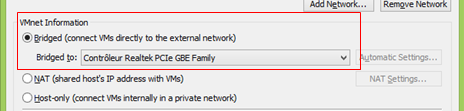
\includegraphics[width=14cm]{img/vmConfig1.png}
		\caption{Configuration de la carte réseau}
		\label{evLinuxConfig1}
	\end{center}
\end{figure}
Puis dans les settings de la VM, il faut aller changer le réseau pour utiliser celui que l’on vient de configurer.
\begin{figure}[H]
	\begin{center}
		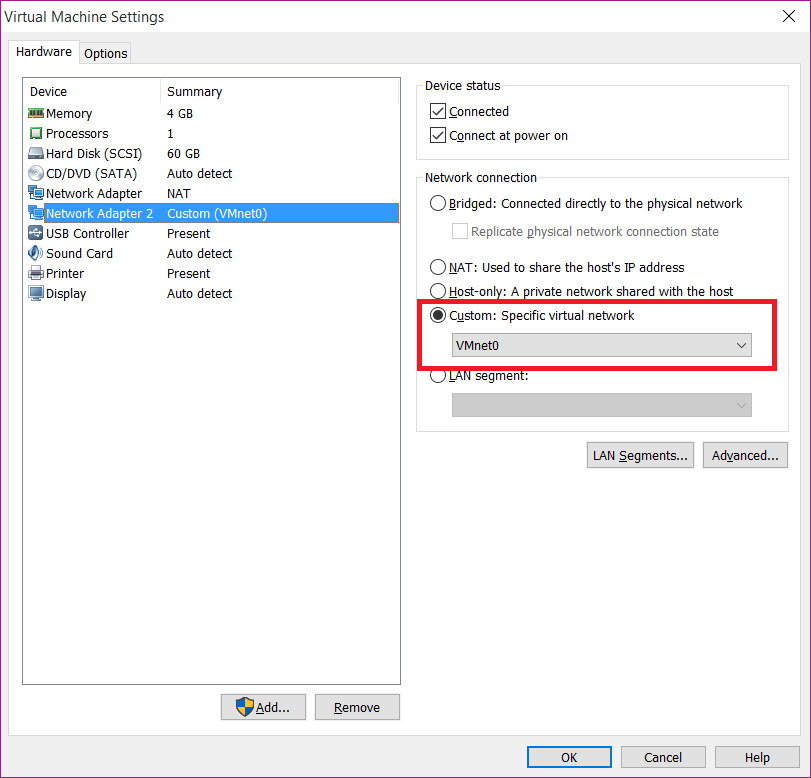
\includegraphics[width=14cm]{img/vmConfig2.png}
		\caption{Association de la carte réseau à la machine virtuelle}
		\label{evLinuxConfig2}
	\end{center}
\end{figure}
La dernière étape est d’activer le réseau dans la machine virtuelle (icône réseau -> enabling networking).
\begin{figure}[H]
	\begin{center}
		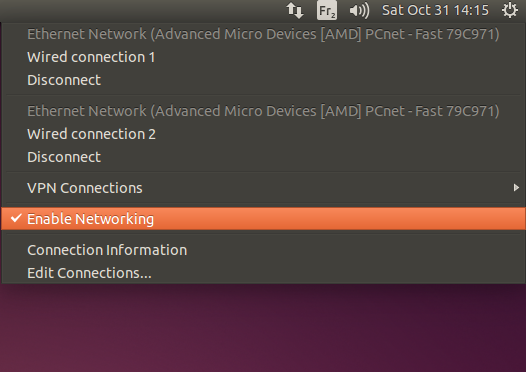
\includegraphics[width=14cm]{img/vmConfig3.png}
		\caption{Activation du réseau}
		\label{evLinuxConfig3}
	\end{center}
\end{figure}

\subsubsection{Accès ssh sans mot de passe}
Il faut aller modifier le fichier \textit{/etc/ssh/sshd\_config} sur la cible pour autoriser l’accès sans mot de passe. Pour accéder au fichier, il faut entrer sur la cible par la connexion série :
\begin{lstlisting}
$ sudo minicom

Welcome to minicom 2.7

OPTIONS: I18n 
Compiled on Jan  1 2014, 17:13:22.
Port /dev/ttyUSB0, 13:10:43

Press CTRL-A Z for help on special keys


Welcome to Hardkernel ODROID_XU3 board
odroidxu3 login: root
# 

\end{lstlisting}
On peut ensuite rechercher le fichier et l’éditer avec vi ou vim pour modifier "PermitEmptyPassword yes". Une fois la configuration faite, il faut redémarrer la cible :
\begin{lstlisting}
# reboot
\end{lstlisting}
Normalement, on devrait avoir accès à la cible en ssh en entrant la commande suivante dans la machine hôte :
\begin{lstlisting}
lmi@csel1:~$ ssh root@192.168.0.11
# 
\end{lstlisting}
Pour valider la connexion Ethernet/IP, on peut également arrêter la cible dans son U-boot en tapant la touche "carriage return" et faire un ping de la machine hôte:
\begin{lstlisting}
lmi@csel1:~$ sudo minicom
...
# reboot
...                                                      
Press 'Enter' or 'Space' to stop autoboot:  0       
                            
ODROIDXU3> usb start                                                            
(Re)start USB...                                                                
USB:   Register 1313 NbrPorts 3                                                 
USB EHCI 1.00                                                                   
scanning bus for devices... The request port(2) is not configured               
The request port(2) is not configured                                           
4 USB Device(s) found                                                           
scanning bus for storage devices... 0 Storage Device(s) found            
scanning bus for ethernet devices... 1 Ethernet Device(s) found          

ODROIDXU3> ping 192.168.0.4                                                     
Waiting for Ethernet connection... done.                                        
Using sms0 device                                                               
host 192.168.0.4 is alive

ODROIDXU3> run nfsboot
\end{lstlisting}
Si la machine hôte répond au ping, tout a bien été configuré.

\subsubsection{Création de l'espace de travail}
Le but est de configurer le noyau Linux afin d’attacher un usrfs sous ext4 depuis la carte SD. En d’autres termes, partager un espace de travail entre la cible et l’hôte. Pour cela, il faut accéder à la cible via le port série ou par ssh et de taper les commandes indiquées dans la donnée.
\begin{lstlisting}
# mkdir /usr/workspace
# vi /etc/fstab
	# /etc/fstab: static file system information.
	#
	# <file system> <mount pt>     <type>   <options>         <dump> <pass>
	/dev/root       /              ext2     rw,noauto         0      1
	proc            /proc          proc     defaults          0      0
	devpts          /dev/pts       devpts   defaults,gid=5,mode=620   0      0
	tmpfs           /dev/shm       tmpfs    mode=0777         0      0
	tmpfs           /tmp           tmpfs    mode=1777         0      0
	sysfs           /sys           sysfs    defaults          0      0
	192.168.0.4:/home/lmi/workspace /usr/workspace  nfs     hard,intr,nolock
# mount -a
# reboot
\end{lstlisting}
Pour contrôler que le répertoire est bien partagé avec la cible, on peut y entrer la commande mount et normalement on voit le répertoire partagé.
\begin{lstlisting}
# mount
...
192.168.0.4:/home/lmi/workspace on /usr/workspace type nfs (rw,relatime,vers=3,rsize=131072,wsize=131072,namlen=255,hard,nolock,proto=tcp,timeo=600,retrans=2,sec=sys,mountaddr=192.168.0.4,mountvers=3,mountproto=tcp,local_lock=all,addr=192.168.0.4)
\end{lstlisting}
\subsection{Debugging de l'application}
Cette section présente les différentes étapes à réaliser pour configurer Eclipse pour qu’il utilise une connexion ssh entre l’hôte et la cible.
Pour cela, il faut commencer par charger un projet dans Eclipse :
\begin{enumerate}
	\item File -> Import… (si le projet existe déjà)
	\item C/C++ ->Existing Code as Makefile Project (configure pour utiliser le Makefile du projet et non un de Eclipse)
	\item Il suffit ensuite de définir le nom du projet et le path jusqu’au code source
\end{enumerate}
Une fois le projet importé dans l’espace de travail, il faut configurer le debugger:
\begin{figure}[H]
	\begin{center}
		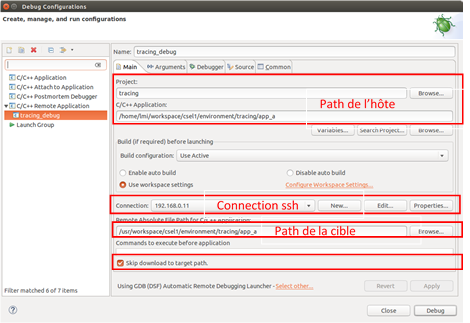
\includegraphics[width=14cm]{img/eclipseConfig1.png}
		\caption{Configuration du debugger}
		\label{eclipseConfig1}
	\end{center}
\end{figure}
Pour pouvoir entrer le path de la cible, il faut impérativement que la connexion ssh soit configurée comme ci-dessous :
\begin{figure}[H]
	\begin{center}
		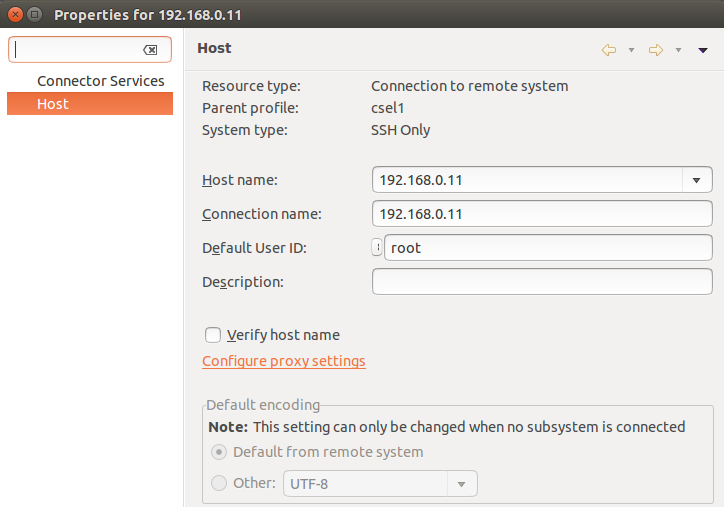
\includegraphics[width=14cm]{img/eclipseConfig2.png}
		\caption{Configuration de l'accès ssh}
		\label{eclipseConfig2}
	\end{center}
\end{figure}
Il faut encore aller configurer le debugger gdb :
\begin{figure}[H]
	\begin{center}
		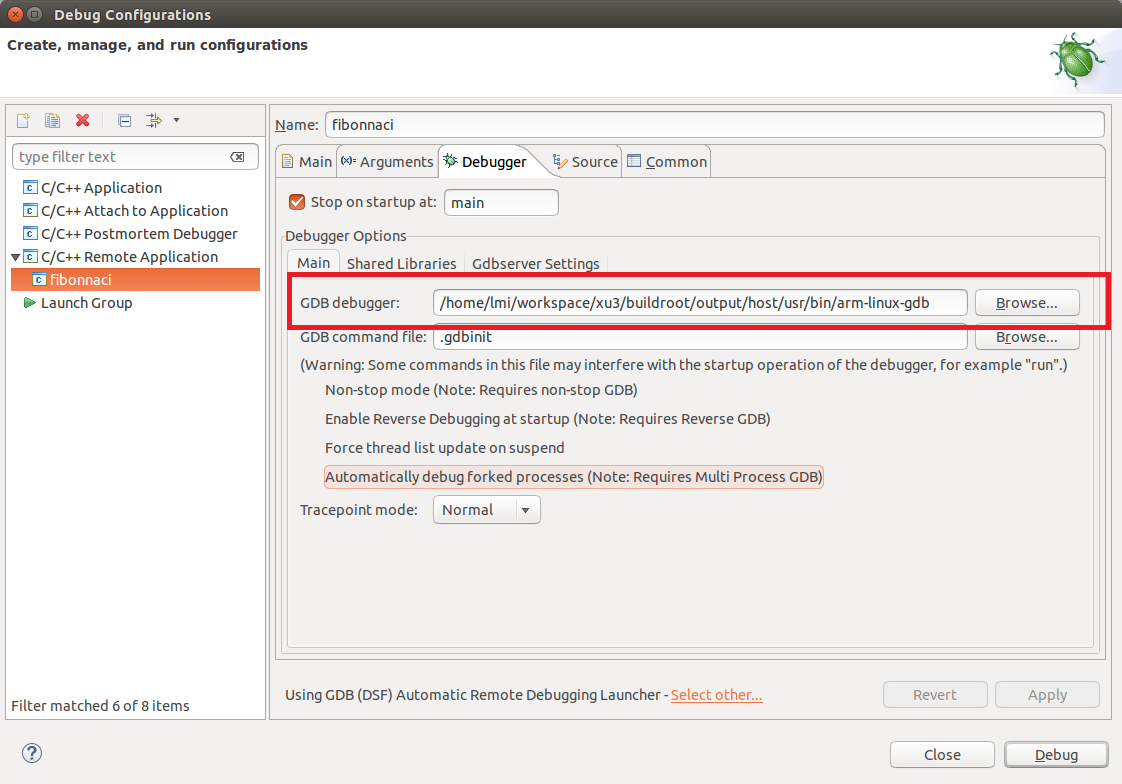
\includegraphics[width=14cm]{img/eclipseConfig3.png}
		\caption{Configuration du server gdb}
		\label{eclipseConfig3}
	\end{center}
\end{figure}
\begin{figure}[H]
	\begin{center}
		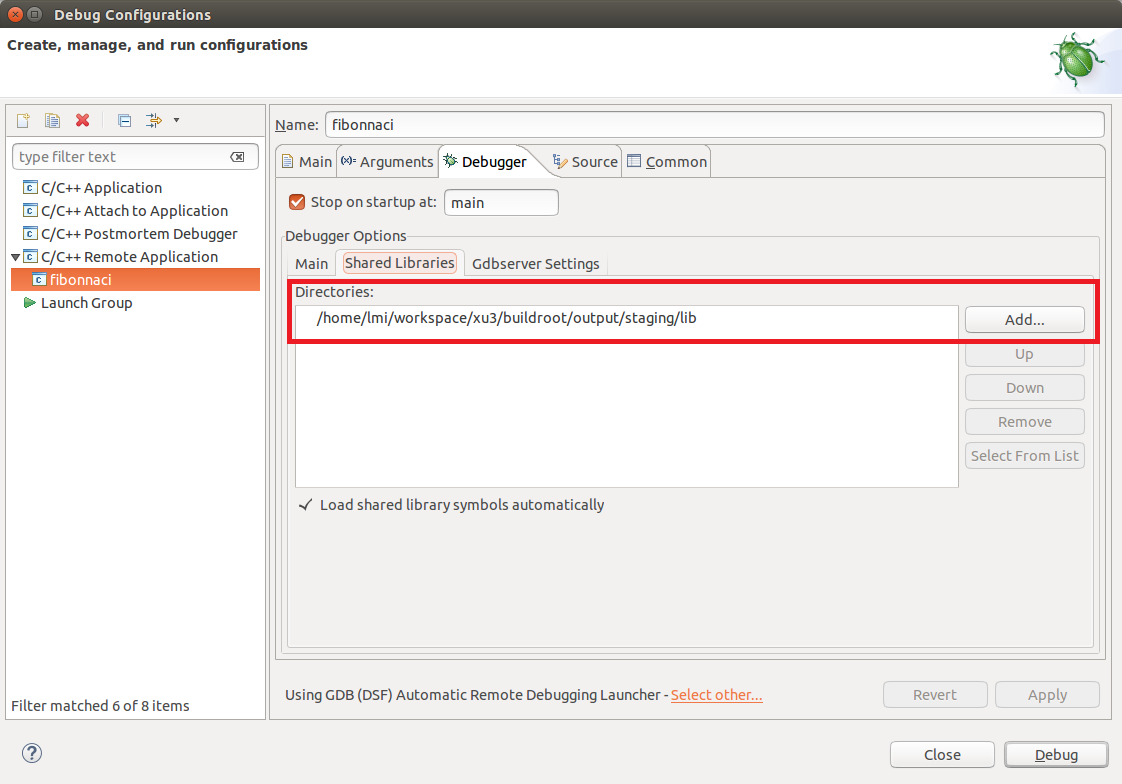
\includegraphics[width=14cm]{img/eclipseConfig4.png}
		\caption{Configuration des shared library}
		\label{eclipseConfig4}
	\end{center}
\end{figure}
Avec cette configuration, on peut ensuite debugger pas à pas les exercices d’exemples. Voici un exemple avec fibonacci:
\begin{figure}[H]
	\begin{center}
		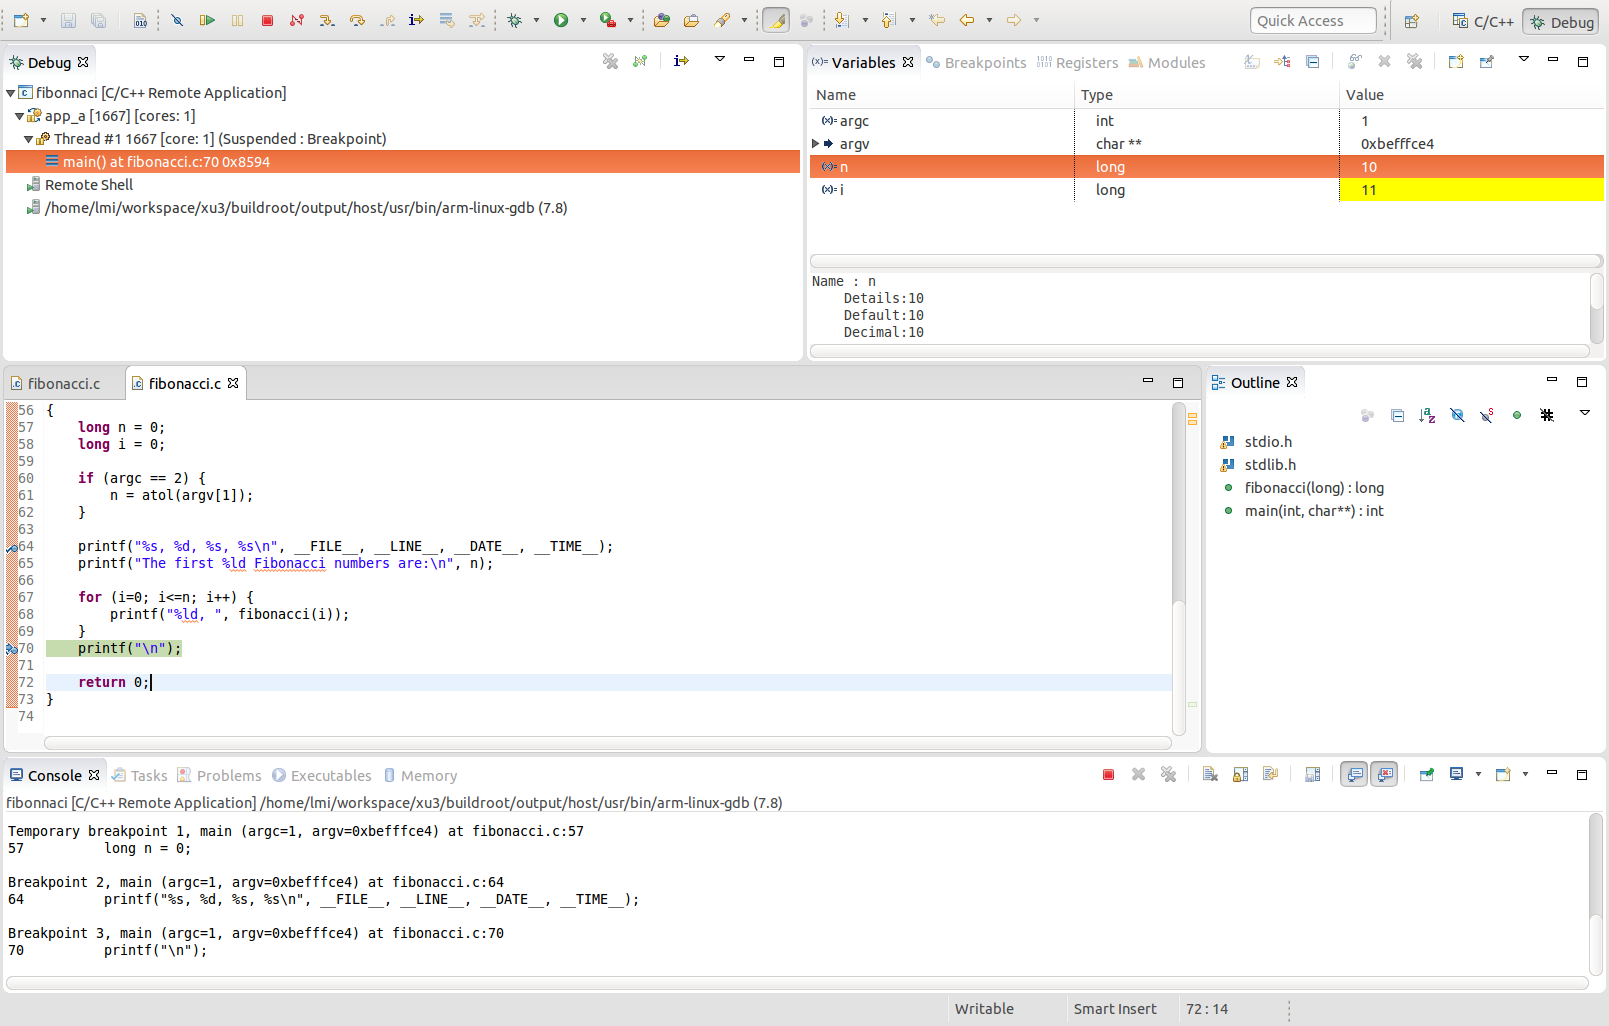
\includegraphics[width=16.5cm]{img/eclipseConfig5.png}
		\caption{Debug de l'exemple Fibonacci}
		\label{eclipseConfig5}
	\end{center}
\end{figure}
\subsection{Test des différents exemples proposés}
Pour la suite du rapport, les symboles suivant sont définis:
\begin{enumerate}
	\item \$ : commande sur la machine hôte
	\item \# : commande sur la cible
	\item > : commande sur la cible arrêtée avant démarrage
\end{enumerate}

\subsubsection{Fibonacci}
\begin{lstlisting}
lmi@csel1:~/workspace/csel1/environment/samples/fibonacci$ make clean all

lmi@csel1:~$ ssh root@192.168.0.11
# cd ../usr/workspace/csel1/environment/samples/fibonacci/
# ./app_a 10
fibonacci.c, 64, Oct 31 2015, 15:27:54
The first 10 Fibonacci numbers are:
0, 1, 1, 2, 3, 5, 8, 13, 21, 34, 55,
\end{lstlisting}

\subsubsection{Tracing}
Avec la trace active
\begin{lstlisting}
lmi@csel1:~/workspace/csel1/environment/samples/tracing$ make DEBUG=1 clean all

# cd ../tracing/
# ./app_a 12
fibonacci.c, 70, Oct 31 2015, 15:35:42
The first 12 Fibonacci numbers are:
0, 1, 1, 2, 3, 5, 8, 13, 21, 34, 55, 89, 144, 
\end{lstlisting}
Avec la trace inactive
\begin{lstlisting}
lmi@csel1:~/workspace/csel1/environment/samples/tracing$ make clean all

# ./app_a 12
The first 12 Fibonacci numbers are:
0, 1, 1, 2, 3, 5, 8, 13, 21, 34, 55, 89, 144, 
\end{lstlisting}

\subsubsection{Core dumps}
\begin{lstlisting}
lmi@csel1:~/workspace/csel1/environment/samples/core_dumps$ make clean all

# cd ../core_dumps/
# ulimit -c unlimited
# ./app_a 
Segmentation fault (core dumped)
# gdb app_a core
...
Core was generated by `./app_a'.
Program terminated with signal SIGSEGV, Segmentation fault.
#0  0x000083e0 in access_data () at core_dumps.c:31
31		*p=10;
(gdb) bt
#0  0x000083e0 in access_data () at core_dumps.c:31
#1  0x00008424 in call (n=0) at core_dumps.c:37
#2  0x00008420 in call (n=1) at core_dumps.c:36
#3  0x00008420 in call (n=2) at core_dumps.c:36
#4  0x00008420 in call (n=3) at core_dumps.c:36
#5  0x00008420 in call (n=4) at core_dumps.c:36
#6  0x00008420 in call (n=5) at core_dumps.c:36
#7  0x00008420 in call (n=6) at core_dumps.c:36
#8  0x00008420 in call (n=7) at core_dumps.c:36
#9  0x00008420 in call (n=8) at core_dumps.c:36
#10 0x00008420 in call (n=9) at core_dumps.c:36
#11 0x00008420 in call (n=10) at core_dumps.c:36
#12 0x00008448 in main () at core_dumps.c:43
\end{lstlisting}


\subsubsection{Backtrace}
Cet exemple s'effectue uniquement sur la machine hôte
\begin{lstlisting}
lmi@csel1:~/workspace/csel1/environment/samples/core_dumps$ cd ../backtrace/
lmi@csel1:~/workspace/csel1/environment/samples/backtrace$ make clean all
...
lmi@csel1:~/workspace/csel1/environment/samples/backtrace$ ./app_h
backtrace() returned 17 addresses
./app_h[0x80484fc]
[0xb7727404]
./app_h[0x804854a]
./app_h[0x8048571]
./app_h[0x804856c]
./app_h[0x804856c]
./app_h[0x804856c]
./app_h[0x804856c]
./app_h[0x804856c]
./app_h[0x804856c]
./app_h[0x804856c]
./app_h[0x804856c]
./app_h[0x804856c]
./app_h[0x804856c]
./app_h[0x804859c]
/lib/i386-linux-gnu/libc.so.6(__libc_start_main+0xf3)[0xb757ca83]
./app_h[0x8048401]
Segmentation fault (core dumped)
lmi@csel1:~/workspace/csel1/environment/samples/backtrace$ addr2line -e app_h 0x804859c
/home/lmi/workspace/csel1/environment/samples/backtrace/main.c:61

\end{lstlisting}
\subsubsection{System calls}
\begin{lstlisting}
lmi@csel1:~/workspace/csel1/environment/samples/system_calls$ make clean all

# cd ../system_calls/
# ./app_a
current temperature: 46.00 degree Celcius

# strace ./app_a
execve("./app_a", ["./app_a"], [/* 21 vars */]) = 0
brk(0)                                  = 0x11000
...
+++ exited with 0 +++

# strace -e trace=mmap2 ./app_a
...
mmap2(NULL, 4096, PROT_READ|PROT_WRITE, MAP_PRIVATE|MAP_ANONYMOUS, -1, 0) = 0xb6ff9000
mmap2(NULL, 4096, PROT_READ|PROT_WRITE, MAP_PRIVATE|MAP_ANONYMOUS, -1, 0) = 0xb6ffa000
current temperature: 47.00 degree Celcius
+++ exited with 0 +++
\end{lstlisting}

\subsubsection{Memory leaks}
\begin{lstlisting}
lmi@csel1:~/workspace/csel1/environment/samples/memory_leaks$ make clean all

# cd ../memory_leaks/
# ./app_a 
# valgrind --leak-check=full ./app_a
==1714== Memcheck, a memory error detector
==1714== Copyright (C) 2002-2013, and GNU GPL'd, by Julian Seward et al.
==1714== Using Valgrind-3.10.0 and LibVEX; rerun with -h for copyright info
==1714== Command: ./app_a
==1714== 
==1714== 
==1714== HEAP SUMMARY:
==1714==     in use at exit: 31,880 bytes in 3,985 blocks
==1714==   total heap usage: 4,000 allocs, 15 frees, 32,000 bytes allocated
==1714== 
==1714== 31,880 (8 direct, 31,872 indirect) bytes in 1 blocks are definitely lost in loss record 2 of 2
==1714==    at 0x483535C: malloc (in /usr/lib/valgrind/vgpreload_memcheck-arm-linux.so)
==1714== 
==1714== LEAK SUMMARY:
==1714==    definitely lost: 8 bytes in 1 blocks
==1714==    indirectly lost: 31,872 bytes in 3,984 blocks
==1714==      possibly lost: 0 bytes in 0 blocks
==1714==    still reachable: 0 bytes in 0 blocks
==1714==         suppressed: 0 bytes in 0 blocks
==1714== 
==1714== For counts of detected and suppressed errors, rerun with: -v
==1714== ERROR SUMMARY: 1 errors from 1 contexts (suppressed: 0 from 0)
\end{lstlisting}

\subsection{Mise en production de l'ODROID-XU3}
\begin{lstlisting}
lmi@csel1:~/workspace/csel1/environment/samples/daemon$ make clean all
\end{lstlisting}
Cette commande génère deux fichiers:
\begin{enumerate}
	\item app\_a
	\item S60appl
\end{enumerate}
Le fichier S60appl a été légèrement modifié pour que le path vers app\_a corresponde:
\begin{lstlisting}
#!/bin/sh
#
# Daemon application
#
case "$1" in
	start)
		/usr/workspace/csel1/environment/samples/daemon/app_a
		;;
	stop)
		killall app_a
		;;
	restart|reload)
		killall app_a
		/usr/workspace/csel1/environment/samples/daemon/app_a
		;;
	*)
		echo $"Usage: $0 {start|stop|restart}"
		exit 1
esac

echo "Daemon application launched"

exit $?
\end{lstlisting}
Il suffit ensuite de copier ce fichier dans \textit{/etc/init.d} et de faire un reboot. Au démarrage de la cible, le script \textit{/etc/init.d/rcs} va effectuer tous les fichiers S?? présent dans le répertoire \textit{/etc/init.d}, donc notre application également.
\begin{lstlisting}
# cp /usr/workspace/csel1/environment/samples/daemon/S60appl /etc/init.d
#reboot
...
Starting logging: OK                                                            
Starting mdev...                                                                
Initializing random number generator... done.                                   
Starting network...                                                             
ip: RTNETLINK answers: File exists                                              
Starting sshd: OK                                                               
Daemon application launched                                                     
[    9.933833] [c4] pwm-samsung: tin parent at 66600000  
\end{lstlisting}
\subsection{Réponse aux questions}
1. Comment faut-il procéder pour générer l'U-Boot?
\begin{lstlisting}

\end{lstlisting}
2. Comment peut-on ajouter et générer un package supplémentaire dans le Buildroot?
\begin{lstlisting}

\end{lstlisting}
3. Comment doit-on procéder pour modifier la configuration du noyau Linux?
\begin{lstlisting}

\end{lstlisting}
4. Comment faut-il faire pour générer son propre RootFS?
\begin{lstlisting}

\end{lstlisting}
5. Comment faut-il procéder pour utiliser la carte eMMC en lieu et place de la carte SD?
\begin{lstlisting}

\end{lstlisting}



\newpage
\section{Programmation noyau : Module noyau}
\subsection{Module noyau}
\subsubsection{Exercice 1}
\textbf{Donnée : } Générer un module noyau "out of tree" pour la cible ODROID-XU3\\
\textbf{Point a :} Créer	le	squelette	d’un	module	noyau	et	générer	le	en	dehors	des	sources	du	noyau	à	l’aide	d’un	Makefile.	Le	module	devra	afficher	un	message	lors	de	son	enregistrement	et	lors	de	sa	désinstallation.\\\\
\textbf{Emplacement du code : } \textit{/ModulesNoyau/exercice1-Module/pointA}\\
Le code a été écrit conformément aux exemples présentés dans le support de cours.\\

\textbf{Exécution du code : } \\
Le code doit être compilé sur la machine hôte à l'aide de la commande suivante:
\begin{lstlisting}
$ make clean all
\end{lstlisting}

\textbf{Point b :} Tester sur la machine hôte la commande "modinfo" sur	votre	skelette de	module et comparer les	informations retournées	avec celles	du	code source.
\begin{lstlisting}
$ modinfo mymodule.ko
filename:       /home/lmi/workspace/csel1/environment/module_noyau/exercice1/pointa/mymodule.ko
license:        GPL
description:    Module Skeleton
author:         Emilie Gsponer
depends:        
vermagic:       3.10.63 SMP preempt mod_unload ARMv7 p2v8 
\end{lstlisting}
Ces informations correspondent à celles entrée dans le skeleton du module:
\begin{lstlisting}
MODULE_AUTHOR("Emilie Gsponer");
MODULE_DESCRIPTION("Module Skeleton");
MODULE_LICENSE("GPL");
\end{lstlisting}
\textbf{Point c :} Installer	le	module (insmod),	contrôler	le	log	du	noyau	(dmesg).\\\\
\textbf{Exécution du code : }Le module doit installé sur la cible à l'aide la commande \textit{insmod}. On peut observer que le module a bien été installé à l'aide de la commande \textit{dmesg}.
\begin{lstlisting}
# insmod mymodule.ko
# dmesg | tail -n 4
[    7.704536] [c5] Freeing unused kernel memory: 436K (c089c000 - c0909000)
[    7.877462] [c4] EXT4-fs (mmcblk0p1): re-mounted. Opts: errors=remount-ro,data=ordered
[    8.967876] [c7] pwm-samsung: tin parent at 66600000
[   53.629226] [c4] Linux module skeleton loaded

\end{lstlisting}
\textbf{Point d :} Comparer	les	résultats	obtenus	par	la	commande	"lsmod"	avec	ceux	obtenus	avec	la	commande	"cat /proc/modules".\\\\
\textbf{Exécution des commandes : } Les deux commandes présentent le même résultat, seule la mise en forme est différente.
\begin{lstlisting}
# cat /proc/modules
mymodule 687 0 - Live 0xbf004000 (O)

# lsmod mymodule.ko
Module                  Size  Used by    Tainted: G  
mymodule                 687  0 
\end{lstlisting}
\textbf{Point e :} Désinstaller	le	module	(rmmod).\\\\
\textbf{Exécution de la commande : } On peut voir à l'aide des commandes \textit{cat /proc/modules}, \textit{lsmod} et \textit{dmesg} que le module a bien été désinstallé.
\begin{lstlisting}
# rmmod mymodule
# cat /proc/modules
# lsmod mymodule.ko
Module                  Size  Used by    Tainted: G  
# dmesg | tail -n 4
[    7.877462] [c4] EXT4-fs (mmcblk0p1): re-mounted. Opts: errors=remount-ro,data=ordered
[    8.967876] [c7] pwm-samsung: tin parent at 66600000
[   53.629226] [c4] Linux module skeleton loaded
[   73.538490] [c5] Linux module skeleton unloaded
\end{lstlisting}

\textbf{Point f :} Adapter	le	Makefile	du	module	pour	autoriser	l’installation	du	module	avec	les	autres	modules	du	noyau	permettant	l’utilisation	de	la	commande	"modprobe".	Le	module	devra	être	installé	dans	le	root	filesystem	utilisé	en	nfs	par	la	cible.\\\\
\textbf{Emplacement du code : } \textit{/ModulesNoyau/exercice1-Module/pointF}\\
Pour que le module puisse être ajouté dans le noyau, il suffit d'ajouter les lignes suivantes au Makefile précédent:
\begin{lstlisting}
MODPATH := /tftpboot/odroidxu3

install:
$(MAKE) -C $(KDIR) M=$(PWD) INSTALL_MOD_PATH=$(MODPATH) modules_install
\end{lstlisting}
\textbf{Exécution du code : }Le code doit être compilé et installé sur la machine hôte à l'aide des commandes suivantes:
\begin{lstlisting}
$ make clean all
$ sudo make install
\end{lstlisting}
Il faut ensuite démarrer la cible en mode nfs pour y installer le module à l'aide de la commande \textit{modprobe}
\begin{lstlisting}
lmi@csel1:~/.ssh$ sudo minicom
...
ODROIDXU3> run nfsboot
(Re)start USB...
...
Welcome to Hardkernel ODROID_XU3 board                                          
odroidxu3 login: root  
# modprobe mymodule                                                             
[   98.024580] [c2] Linux module skeleton loaded                                
# modprobe -r mymodule                                                          
[   99.673514] [c0] Linux module skeleton unloaded   
\end{lstlisting}
\subsubsection{Exercice 2}
\textbf{Donnée : } Adapter	le	module	de	l’exercice	précédent	afin	qu’il	puisse	recevoir	deux	ou	trois paramètres de	votre	choix.	Ces	paramètres	seront	affichés dans	la	console.	Adapter	également	le rootfs	afin	de	pouvoir	utiliser	la	commande	"modprobe".\\\\
\textbf{Emplacement du code : } \textit{/ModulesNoyau/exercice1-Module/exercice2-Parameter}\\\\
\textbf{Exécution du code : }Ce module prend deux paramètres d'entrée par défaut, text = "hello" et elements = 2. La valeur de ces éléments peut être modifiée lors de l'installation du module dans le noyau, comme le montre la démonstration suivante.
\begin{lstlisting}
# modprobe mymodule                                                             
[  922.323941] [c1] Linux module skeleton loaded                                
[  922.326835] [c1] text:hello                                                  
[  922.326835] elements:2                                                       
# modprobe -r mymodule                                                          
[  925.223513] [c0] Linux module skeleton unloaded                         
# modprobe mymodule text="hello world" elements=10                              
[ 1196.597223] [c2] Linux module skeleton loaded                                
[ 1196.600182] [c2] text:hello world                                            
[ 1196.600182] elements:10                                                      
# modprobe -r mymodule                                                          
[ 1199.518513] [c0] Linux module skeleton unloaded  
\end{lstlisting}
\textbf{Remarque : } Pour tous les exercices suivants, on reprendra le même Makefile permettant d'installer le module directement dans le noyau à l'aide de la commande \textit{modprobe}. Il faudra pour cela que la cible soit démarrée en mode nfs. Le module de chaque exercice devra être compilé et installé à l'aide des commandes suivantes:
\begin{lstlisting}
$ make clean all
$ sudo make install
\end{lstlisting}
\subsubsection{Exercice 3}
\textbf{Donnée : } Trouver	la	signification	des	4	valeurs	affichées	lorsque	l’on	tape	la	commande "cat /proc/sys/kernel/printk".\\\\
\textbf{Exécution de la commande : }
\begin{lstlisting}
# cat /proc/sys/kernel/printk                                                   
10      4       1       7 
\end{lstlisting}
Ces chiffres représentent le log level du kernel utilisé pour déterminer l'importance d'un message.
\begin{enumerate}
	\item 10 : current loglevel
	\item 4 : default loglevel
	\item 1 : minimum loglevel
	\item 7 : boot-time-default loglevel
\end{enumerate}
Cela permet de définir la priorité des messages. Si un message a une priorité plus grande (chiffre plus petit) que le loglevel courant du kernel, il sera affiché dans la console. Dans le cas contraire, le message n'est pas affiché.L'exemple suivant le démontre en passant le loglevel à 1, le module n'affiche plus de message dans la console.
\begin{lstlisting}
# echo 10 > /proc/sys/kernel/printk                                             
# cat /proc/sys/kernel/printk                                                   
10      4       1       7                                                       
# modprobe mymodule                                                             
[ 2139.129459] [c2] Linux module skeleton loaded                                
[ 2139.132348] [c2] text:hello                                                  
[ 2139.132348] elements:2                                                       
# modprobe -r mymodule                                                          
[ 2143.683511] [c0] Linux module skeleton unloaded        
                      
# echo 1 > /proc/sys/kernel/printk                                              
# cat /proc/sys/kernel/printk                                                   
1       4       1       7                                                       
# modprobe mymodule                                                             
# modprobe -r mymodule     
                                                     
# echo 10 > /proc/sys/kernel/printk                                             
# modprobe mymodule                                                             
[ 2173.021095] [c2] Linux module skeleton loaded                                
[ 2173.024050] [c2] text:hello                                                  
[ 2173.024050] elements:2    
\end{lstlisting}  
Source : \url{http://elinux.org/Debugging_by_printing}

\subsection{Gestion de la mémoire, bibliothèques et fonctions utiles}
\subsubsection{Exercice 4}
\noindent
\textbf{Donnée : }Créer dynamiquement des éléments dans le noyau. Adapter un module noyau afin que l'on puisse lors de son installation spécifier un nombre d'éléments à créer ainsi qu'un texte initial à stocker dans les éléments précédemment alloués. Chaque élément contiendra également un numéro unique, Les éléments seront créés lors de l'installation du module et chainés dans une liste. Ces éléments seront détruits lors de la désinstallation du module. Des messages d'information seront émis afin de permettre le debugging du module.\\\\
\textbf{Emplacement du code : } \textit{/ModulesNoyau/exercice4-List}\\\\
\textbf{Exécution du code : }
\begin{lstlisting}
# modprobe mymodule element_num=5 text="Hello world"                            
[ 2250.418060] [c2] New element added to the list                               
[ 2250.421107] [c2] New element added to the list                               
[ 2250.425536] [c2] New element added to the list                               
[ 2250.429937] [c2] New element added to the list                               
[ 2250.434368] [c2] New element added to the list                               
[ 2250.438773] [c2] ID of element : 0                                           
[ 2250.438773] String is : Hello world                                          
[ 2250.445642] [c2] ID of element : 1                                           
[ 2250.445642] String is : Hello world                                          
[ 2250.452489] [c2] ID of element : 2                                           
[ 2250.452489] String is : Hello world                                          
[ 2250.459415] [c7] ID of element : 3                                           
[ 2250.459415] String is : Hello world                                          
[ 2250.466444] [c7] ID of element : 4                                           
[ 2250.466444] String is : Hello world                                          
# modprobe -r  mymodule                                                         
[ 2267.933575] [c1] Element poped                                               
[ 2267.935161] [c1] Element poped                                               
[ 2267.938196] [c1] Element poped                                               
[ 2267.941283] [c1] Element poped                                               
[ 2267.944313] [c1] Element poped                                               
[ 2267.947308] [c1] Module removed
\end{lstlisting}
\subsubsection{Exercice 5}
\noindent
\textbf{Donnée : }Indiquer les différents alocateurs SLAB disponibles dans le noyau Linux pour la cible ORDOID-XU3
\begin{enumerate}
	\item SLAB : "as cache frendly as possible, benchmark frendly"
	\item SLOB : "as compact as possible"
	\item SLUB : "Simple and instruction cost counts. Superior Debugging. Defragmentation. Execution time friendly"
\end{enumerate}
Source : \url{https://www.google.ch/url?sa=t&rct=j&q=&esrc=s&source=web&cd=3&cad=rja&uact=8&ved=0CDEQFjACahUKEwiqj6GfhKbIAhWLXBoKHXDUAow&url=http%3A%2F%2Fwww.cs.berkeley.edu%2F~kubitron%2Fcourses%2Fcs194-24-S14%2Fhand-outs%2Fbonwick_slab.pdf&usg=AFQjCNENx6yGi8dVRbdR2Si1OpXE_NuNkg&sig2=ZdJ_jUWHIfO1qFIIikEyHA}
	
\subsection{Accès aux entrées/sorties}
\subsubsection{Exercice 6}
\textbf{Donnée : }À l'aide d'un module noyau, réserver la zone mémoire correspondante au registre du uP décrivant son identification. Adress de départ 0x1000'0000, taille de la zone 0x100. Valider cette réservation à l'aide de la commande "cat /proc/iomem".\\
\\
Adapter ce module afin d'afficher cet identifiant dans la console de déboggage "dmesg". Ce dernier est composé des champs suivants:
\begin{enumerate}
	\item Bit 31..12: product id
	\item Bit 11..8: package id
	\item Bit 7..4: major revision
	\item Bit 3..0: minor revision\\
\end{enumerate}
\textbf{Emplacement du code : } \textit{/ModulesNoyau/exercice6-IO}\\\\
\textbf{Complément : }L'identifiant demandé par la donnée est en fait l'identifiant de la zone mémoire réservée. Il peut être obtenu grâce à la méthode \textit{ioread}. Mais pour pouvoir lire cette zone, il faut la mapper dans la mémoire virtuelle du noyau avec la méthode \textit{ioremap}, car le noyau n'a pas directement accès aux entrées/sorties.\\
La zone mémoire réservée par le code a été nommée "uP register".\\\\
\textbf{Exécution du code : }
\begin{lstlisting}
# modprobe mymodule                                                             
[   30.336553] [c5] Linux module skeleton loaded                                
[   30.339495] [c5] Memory allocated                                            
[   30.342733] [c5] uP register: Bit 31..12 : product id=0x65422                
[   30.348494] [c5] uP register: Bit 11..8  : package id=0x0                    
[   30.353877] [c5] uP register: Bit 7..4   : major revision=0x0                
[   30.359597] [c5] uP register: Bit 3..0   : minor revision=0x1                
# cat /proc/iomem                                                               
03000000-03048fff : /lpass@03810000                                             
03810000-038100ff : /lpass@03810000                                             
03830000-038300ff : samsung-i2s                                                 
03860000-03860fff : /pinctrl@03860000                                           
03880000-03880fff : /amba/adma@03880000                                         
03880000-03880fff : /amba/adma@03880000                                      
10000000-100000ff : uP register                                                 
...                                             
# dmesg |tail -n 10                                                             
[    9.041140] [c4] VFS: Mounted root (nfs filesystem) on device 0:13.          
[    9.048765] [c4] devtmpfs: mounted                                           
[    9.050869] [c4] Freeing unused kernel memory: 436K (c089c000 - c0909000)    
[   12.571761] [c4] pwm-samsung: tin parent at 66600000                         
[   30.336553] [c5] Linux module skeleton loaded                                
[   30.339495] [c5] Memory allocated                                            
[   30.342733] [c5] uP register: Bit 31..12 : product id=0x65422                
[   30.348494] [c5] uP register: Bit 11..8  : package id=0x0                    
[   30.353877] [c5] uP register: Bit 7..4   : major revision=0x0                
[   30.359597] [c5] uP register: Bit 3..0   : minor revision=0x1                
# modprobe -r  mymodule                                                         
[   88.338556] [c0] Linux module skeleton unloaded                              
[   88.341621] [c0] Memory released    
\end{lstlisting}

\subsection{Threads du noyau}
\subsubsection{Exercice 7}
\textbf{Donnée : }Développer	un	petit	module	permettant	d’instancier	un	thread	dans	le	noyau.	Ce	thread	affichera	un	message	toutes	les	5	secondes.	Il	pourra	être	mis	en	sommeil	durant	ces	5	secondes à	l’aide	de	la	fonction	« ssleep(5) »	provenant	de	l’interface	<linux/delay.h>.\\\\
\textbf{Emplacement du code : } \textit{/ModulesNoyau/exercice7-Thread}\\\\
\textbf{Exécution du code : }
\begin{lstlisting}
# modprobe mymodule                                                             
[ 1434.469821] [c2] Thread created                                              
# [ 1439.473573] [c1] Thread awake                                              
[ 1444.478588] [c2] Thread awake                                                
[ 1449.483589] [c3] Thread awake                                                
# modprobe -r  mymodule                                                         
[ 1454.488597] [c0] Thread awake                                                
[ 1454.490139] [c1] Thread stopped   
\end{lstlisting}
\subsection{Mise en sommeil}
\subsubsection{Exercice 8}
\textbf{Donnée : }Développer	un	petit	module	permettant	d’instancier	deux threads dans	le	noyau.	Le	premier	thread	attendra	une	notification	de	réveil	du	deuxième	thread et	se	remettra	en sommeil.	Le	2ème thread	enverra	cette	notification	toutes	les	5	secondes	et	se	rendormira. On	utilisera	les	waitqueues pour	les	mises	en	sommeil.	Afin	de	permettre	le	debugging	du	module,	chaque	thread	affichera	un	petit	message	à	chaque	réveil.\\\\
\textbf{Emplacement du code : } \textit{/ModulesNoyau/exercice8-MiseEnSommeil}\\\\
\textbf{Exécution du code : }
\begin{lstlisting}
# modprobe mymodule                                                             
[ 1523.052680] [c2] Init wait queue                                             
[ 1523.054851] [c2] Threads created                                             
# [ 1528.058588] [c3] Thread2 (notif each 5s) awake                             
[ 1528.061596] [c1] Thread1 (wait notif) awake                                  
[ 1533.063590] [c0] Thread2 (notif each 5s) awake                               
[ 1533.066587] [c1] Thread1 (wait notif) awake                                  
[ 1538.068588] [c0] Thread2 (notif each 5s) awake                               
[ 1538.071587] [c1] Thread1 (wait notif) awake                                  
# modprobe -r  mymodule                                                         
[ 1543.073563] [c0] Thread2 (notif each 5s) awake                               
[ 1543.076562] [c2] Thread1 (wait notif) awake                                  
[ 1548.078569] [c0] Thread2 (notif each 5s) awake                               
[ 1548.081573] [c1] Threads stopped  
\end{lstlisting}
\subsection{Gestion des interruptions}
\subsubsection{Exercice 9}
\textbf{Donnée : }Développement d'un petit module permettant de capturer les pressions exercées sur les swtiches de la carte d'extension par interruption. Afin de permettre le debugging du module, chaque capture affichera un petit message.\\
Informations fournies:
\begin{itemize}
	\item Configurer la direction des GPIO en entrée : 
	\begin{lstlisting}
	gpio_resquest(EXYNOS5_GPX<gpio_nr>(<pin-nr>));
	\end{lstlisting}
	\begin{lstlisting}
	gpio_direction_input(EXYNOS5_GPX<gpio_nr>(<pin_nr>));
	\end{lstlisting}
	\item Obtenir le vecteur d'interruption avec le service suivant:
	\begin{lstlisting}
	gpio_to_irq (<io_nr>);
	\end{lstlisting}
	\item Informations sur les switches de la carte d'extension 
	\begin{itemize}
	\item sw1 - gpio\_nr=2, pin\_nr=5,  io\_nr=29
	\item sw2 - gpio\_nr=2, pin\_nr=6,  io\_nr=30
	\item sw3 - gpio\_nr=1, pin\_nr=6,  io\_nr=22
	\item sw4 - gpio\_nr=1, pin\_nr=2,  io\_nr=18\\
	\end{itemize}
\end{itemize}
\textbf{Complément : } Les switches de 1 à 4 sont interceptés. \\\\
\textbf{Emplacement du code : } \textit{/ModulesNoyau/exercice9-Interrupt}\\\\
\textbf{Exécution du code : }
Et voici la preuve que tout fonctionne conformément, avec un message s'affichant pour chaque bouton pressé:
\begin{figure}[H]
	\begin{center}
		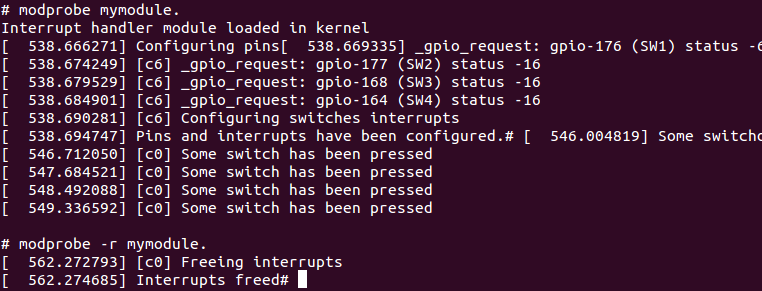
\includegraphics[width=14cm]{img/interrupt_success.png}
		\caption{Affichage du chargement du module, des pressions sur les boutons et de la suppression du module}
		\label{ser1ex9}
	\end{center}
\end{figure}

\section{Programmation noyau : Pilotes de périphériques}
\subsection{Pilotes orientés mémoire}
\subsubsection{Exercice 1}
\textbf{Donnée : } Réaliser	un	pilote	orienté	mémoire	permettant	de	mapper	en	espace	utilisateur	les	registres	de	la	
 FPGA	en	utilisant	le	fichier	virtuel	\textit{/dev/mem}.	Ce	pilote	permettra	de	lire	l’identification	du	uP	
(chip	id)	décrit	dans	l’exercice	no 6 du	cours	sur	la	programmation	de	modules	noyau.\\\\
\textbf{Complément : } Ce pilote n'est pas un module noyau, il faut prendre le Makefile d'un des codes d'exemples, par exemple Fibonacci. La cible doit tout de même être démarrée en mode nfs.\\\\
\textbf{Emplacement du code : } \textit{/PilotesPeripheriques/exercice1-mmap}\\

\textbf{Exécution du code : } \\
\begin{lstlisting}
# ./app_a                                                                       
uP register: Bit 31..12 : product id=0x65422                                    
uP register: Bit 11..8  : package id=0x0                                        
uP register: Bit 7..4   : major revision=0x0                                    
uP register: Bit 3..0   : minor revision=0x1 
\end{lstlisting}

\textbf{Remarque : } On obtient bien le même id qu'avec le module noyau de l'exercie 6 de la série précédente.\\
Pour utiliser correctement la commande mmap, il ne faut pas mettre l'offset à 0, mais à 0x1000000 (adresse du chipid de l'exercice6), sinon le code ne fonctionne pas, il essaie de lire une zone mémoire qu'il n'a pas le droit.

\subsubsection{Exercice 2}
\textbf{Donnée : } Sur	la	base	de	l’exercice	1,	développer	un	pilote	orienté	caractère	permettant	de	mapper	en	
espace	utilisateur	ces registres	(implémentation	de	l’opération	de	fichier	« mmap »).	
Le	driver	orienté	mémoire	sera	ensuite	adapté	à	cette	nouvelle	interface.
Remarque :	à	effectuer	après	les	exercices	des	pilotes	orientés	caractère\\\\
\textbf{Emplacement du code : }\\ \textit{/PilotesPeripheriques/exercice2-mmapModule/user}\\
\textit{/PilotesPeripheriques/exercice2-mmapModule/noyau}\\

\textbf{Remarque : }Cet exercice a été compliqué à réaliser. Le code est un mélange de l'exercice 1 et 5. Il faut garder en tête que pour mapper les registres en espace utilisateur, il faut utiliser les fonction standard des file\_operations (open,close,mmap) et en plus, ajouter les vm\_operations\_struct (open,close) pour agir sur la zone mémoire. Dans le pilote orienté caractère, on utilise la fonction \textit{remap\_pfn\_range} pour mapper la zone mémoire.\\

\textbf{Exécution du code : } \\
\begin{lstlisting}
# modprobe mymodule                                                             
[  854.599130] [c2] mod: successfully loaded with major 249                     
# mknod /dev/mod c 249 0    
# ./app_a /dev/mod                                                              
[ 1166.619318] [c0] mod: open                                                   
[ 1166.620800] [c0] mod: mmap                                                   
[ 1166.623246] [c0] VMA open, virt b6f71000, phys 10000000                      
[ 1166.628986] [c0] VMA close.                                                  
[ 1166.631259] [c0] mod: release                                                
file /dev/mod open                                                              
Physical memory: Bit 31..12 : product id=0x65422                                
Physical memory: Bit 11..8  : package id=0x0                                    
Physical memory: Bit 7..4   : major revision=0x0                                
Physical memory: Bit 3..0   : minor revision=0x1                                

Virtual memory: Bit 31..12 : product id=0x43108                                 
Virtual memory: Bit 11..8  : package id=0x3                                     
Virtual memory: Bit 7..4   : major revision=0x2                                 
Virtual memory: Bit 3..0   : minor revision=0xa                                 
file /dev/mod close 
# modprobe -r mymodule                                                          
[ 1259.338388] [c0] mod: successfully unloaded   
\end{lstlisting}

\subsection{Pilotes orientés caractères}
\subsubsection{Exercice 3}
\textbf{Donnée : } Implémenter	un	pilote	de	périphérique	orienté	caractère.	Ce	pilote	sera	capable	de	stocker	dans	
une	variable	globale	au	module	les	données	reçues	par	l’opération	write et	de	les	restituer	par	
l’opération	read. Pour	tester	le	module,	on	utilisera	les commandes « echo » et	« cat ».\\\\
\textbf{Emplacement du code : } \textit{/PilotesPeripheriques/exercice3-ReadWrite}\\

\textbf{Exécution du code : } \\
\begin{lstlisting}
$ make clean all
$ sudo make install
\end{lstlisting}
\begin{lstlisting}
# modprobe mymodule                                                             
[ 4107.528630] [c2] mod: successfully loaded with major 249                     
# mknod /dev/mod c 249 0                                                        
# echo -n test module > /dev/mod                                                
[ 4134.907095] [c1] mod: open()                                                 
[ 4134.908540] [c1] mod: write test module                                      
[ 4134.912539] [c1] mod: release()                                              
# cat /dev/mod                                                                  
[ 4145.581863] [c0] mod: open()                                                 
[ 4145.583312] [c0] mod: read test module                                       
[ 4145.587140] [c0] mod: read test module                                       
[ 4145.590820] [c0] mod: release()                                              
# modprobe -r  mymodule                                                         
[ 4157.528779] [c1] mod: successfully unloaded   
\end{lstlisting}

\subsubsection{Exercice 4}
\textbf{Donnée : } Etendre	la	fonctionnalité	du	pilote	de	l’exercice	\#3 afin	que	l’on	puisse	à	l’aide	d’un	paramètre	
module	spécifier	le	nombre	d’instance.	Pour	chaque	instance	on	créera	une	variable	unique	
permettant	de	stocker	les	données	échangées	avec	l’application	en	espace	utilisateur.\\\\
\textbf{Emplacement du code : } \textit{/PilotesPeripheriques/...}\\

\textbf{Exécution du code : } \\
\begin{lstlisting}

\end{lstlisting}

\subsubsection{Exercice 5}
\textbf{Donnée : } Développer	une	petite	application	en	espace	utilisateur	permettant	d’accéder	à	ces	pilotes	
orientés	caractère.	L’application	devra	écrire	un	texte	dans	le	pilote	et	le	relire.\\\\
\textbf{Complément : } Le module noyau a été repris de l'exercice 3.\\\\
\textbf{Emplacement du code : }\\ \textit{/PilotesPeripheriques/exercice5-UserAccess/user}\\
\textit{/PilotesPeripheriques/exercice5-UserAccess/noyau}\\

\textbf{Exécution du code : } \\
\begin{lstlisting}
lmi@csel1:~/workspace/csel1/environment/peripheral/exercice5/user$ make clean all
lmi@csel1:~/workspace/csel1/environment/peripheral/exercice5/user$ cd ../noyau/
lmi@csel1:~/workspace/csel1/environment/peripheral/exercice5/noyau$ make clean all
lmi@csel1:~/workspace/csel1/environment/peripheral/exercice5/noyau$ sudo make install
\end{lstlisting}
\begin{lstlisting}
# modprobe mymodule                                                             
[  231.111019] [c2] mod: successfully loaded with major 249    
# mknod /dev/mod c 249 0                  
# ./app_a /dev/mod HELLO                                                        
[  234.969067] [c0] mod: open()                                                 
[  234.970719] [c0] mod: write HELLO                                            
[  234.973927] [c0] mod: read HELLO                                             
[  234.977039] [c0] mod: release()                                              
file /dev/mod open                                                              
write HELLO                                                                     
read HELLO                                                                      
file /dev/mod close                                                             
# modprobe -r mymodule                                                          
[  261.512478] [c0] mod: successfully unloaded
\end{lstlisting}

\subsection{Opérations bloquantes}
\subsubsection{Exercice 6}
\textbf{Donnée : } Développer	un pilote	et	une	application	utilisant	les	entrées/sorties	bloquantes	pour	signaler	une	
interruption	matérielle provenant	de	l’un	des	switches	de	la	carte	d’extension	de	ODROID-XU3.
L’application	utilisera	le	service	select	pour	compter	le	nombre	d’interruptions.\\
\textit{Remarque :	les	switches	non	pas	d’anti-rebond,	par	conséquent il	est	fort	probable	que	vous	
comptiez	un	peu	trop	d’impulsions ;	effet	à	ignorer.	}
\\\\
\textbf{Emplacement du code : } \textit{/PilotesPeripheriques/...}\\

\textbf{Exécution du code : } \\
\begin{lstlisting}

\end{lstlisting}

\subsection{sysfs}
\subsubsection{Exercice 7}
\textbf{Donnée : } Développer	un	pilote	de	périphérique	orienté	caractère	permettant	de	valider	la	fonctionnalité	du	
sysfs.	Le	pilote		offrira	des	attributs	de	périphérique	afin	pouvoir	lire	et	écrire	un	bloc	de	données	
composé	de	quelques	membres	et	de	pouvoir	modifier	le	contenu	de	la	valeur	entière.	Seules	les	
commandes	« echo » et	« cat » doivent	être	nécessaire	pour	manipuler	ces	attributs.\\\\
\textbf{Emplacement du code : } \textit{/PilotesPeripheriques/...}\\

\textbf{Exécution du code : } \\
\begin{lstlisting}

\end{lstlisting}

\subsection{ioctl (optionnel)}
\subsubsection{Exercice 8}
Cet exercice n'a pas été réalisé.

\subsection{procfs (optionnel)}
\subsubsection{Exercice 9}
Cet exercice n'a pas été réalisé.

\subsection{Gestionnaires de périphériques}
\subsubsection{Exercice 10}
\textbf{Donnée : } Implémenter	à	l’intérieur	d’un	pilote	de	périphérique	orienté	caractère,	les	mécanismes	
nécessaires	à	la	création	du	fichier	d’accès	au	pilote	(remplacement	de	la	commande	« mknod »)	
par	l’utilitaire	« mdev »	de	la	BusyBox.\\\\
\textbf{Emplacement du code : } \textit{/PilotesPeripheriques/...}\\

\textbf{Exécution du code : } \\
\begin{lstlisting}

\end{lstlisting}









\section{Programmation système : Système de fichiers}
\subsection{Contexte}
La	carte ODROID-XU3	Lite	est	équipé	d’un	petit	ventilateur	afin	d’évacuer	la	chaleur	produite	par	
l’activité	du	microprocesseur.	La	vitesse	du	ventilateur	est	contrôlée par	un	PWM	(Pulser-Width	
Modulation),	dont	le	rapport	de	cycle	(duty)	dépendra	de	la	température	du	microprocesseur.	Le	
ventilateur	sera	régulé	sur	la	base	de	20kHz.		Sur	la	carte	ODROID-XU3	Lite	ce	PWM	peut	être	réalisé	
avec	la	porte	d’entrée/sortie	"gpb2\_0".
\subsection{Travail à réaliser}
Sur	le	site	moodle	vous	trouverez	une	petite	application	qui	contrôle	la	vitesse	du	ventilateur.	Ce	code	
n’a	pas	été	très	bien	programmé	et	utilise	le	100\%	d’un	cœur	du	processeur	(à	mesurer	avec	top).	
Concevez	une	application	permettant	de	gérer	la	vitesse	de	rotation	du	ventilateur	de	l’ODROID-XU3	
à	l’aide	des	trois	boutons	poussoir.
Quelques	indications	pour	la	réalisation de	l’application :
\begin{enumerate}
\item Au	démarrage	le	duty	cycle	du	ventilateur	sera	réglé	à	50\%
\item Utilisation	des	boutons	poussoir
\begin{enumerate}
\item « sw1 »	pour	augmenter	la	vitesse	du	ventilateur
\item « sw2 »	pour	remettre	la	vitesse	du	ventilateur	à	sa	valeur	initiale
\item « sw3 »	pour	diminuer	la	vitesse	du	ventilateur
\item une	pression	continue	exercée	sur	un	bouton	indiquera	une	auto	incrémentation	
ou	décrémentation	du	duty	cyle.
\end{enumerate}
\item Tous	les	changements	de	vitesse	du	ventilateur	seront	logger	avec	syslog	de	Linux.
\item Le	multiplexage	des	entrées/sorties	devra	être	utilisé.
\end{enumerate}

\subsection{Travail réalisé}
\subsubsection{Description}
Tous les points de la donnée ont été implémentés. La fréquence du ventilateur a été augmentée à 50 kHz, car à 20kHz le ventilateur émet un son strident très agaçant.\\Pour le point de l'auto incrémentation, la duty cycle est augmenté/diminué de 2\% chaque 40 us quand un bouton est maintenu appuyé. Si par hasard, on maintient appuyé deux boutons en même temps, le programme attend qu'un des deux soit relâché pour changer le duty cycle.\\En plus des points demandés, les LEDs de la carte d'extensions sont utilisées.
\begin{enumerate}
	\item LED1: S'allume et s'éteint en fonction de la pression sur le switch 1.
	\item LED2 : Clignote à la fréquence de la PWM. La vitesse est trop rapide pour la voir clignoter, on peut par contre observer un changement de luminosité entre un duty cycle proche de 0\% et un proche de 100\%.
	\item LED3 : S'allume et s'éteint en fonction de la pression sur le switch 3.\\
\end{enumerate} 

\textbf{Emplacement du code : } \textit{/FanControl}

\subsubsection{Configuration des GPIO}

\subsubsection{Exécution du code}

\subsubsection{Syslog}

\subsubsection{Mesure de performance}

\subsubsection{Amélioration possibles}
Les switch n'ont pas d'anti-rebond. Parfois, l'état du bouton du programme ne correspond pas à l'état physique du bouton. La conséquence est que le duty cylcle s'incrémente/décrémente alors qu'aucun bouton n'est appuyé. Il faudrait implémenter un anti-rebond software. Ce point n'a pas été réalisé, car ce n'était pas l'objectif du labo. Si le problème se présente, il suffit de relancer le programme.

\end{document}


